\chapter{Tree decomposition}

A \emph{tree decomposition} of a (connected) graph $G$ is a tree $T$ such that
\begin{enumerate}
    \item each vertex $v$ of the graph $G$ is contained in a vertex (bag) of $T$,
    \item for each edge $uv$ of the graph $G$, there is a vertex (bag) of $T$ that contains both $u$ and $v$,
    \item for each vertex $v$ of $G$, the set of vertices of $T$ which contain $v$ induce a connected subtree.
\end{enumerate}

\section{Exercises}

\subsection{Bucket elimination}

Bucket elimination is a heuristic algorithm for finding a tree decomposition for a graph $G$.

\medskip
\noindent \textbf{Algorithm:}
Order the vertices of $G$ by non-increasing degree
\begin{enumerate}
    \item for each vertex $v \in V(G)$ add a vertex to $T$ with the initial bag $B(v)$ containing $v$,
    \item for each edge $uv \in E(G)$ add the "left" vertex to the bag of the "right" vertex,
    \item From right to left process the vertices $v$:
    \begin{enumerate}
        \item let $A$ be the bag $B(v) \setminus \{v\}$,
        \item let $u$ be the rigthmost vertex in $A$,
        \item add $A$ to the bag $B(u)$ and add  edge $uv$ to the tree.
    \end{enumerate}
\end{enumerate}

Write a function \verb`bucket_elimination(G)` which returns a tree decomposition of $G$ computed by the bucket elimination algorithm.
Also, write a function \verb`decomposition_width(B)` which returns the width of the tree decomposition $B$, $B$ is a bucket map returned by the function \verb`bucket_elimination`. Compare with the value returned by the Sage function \verb`treewidth()`.

\subsubsection*{Solution and tests}
\begin{sageCell}
def bucket_elimination(G):
    """
    Bucket elimination algorithm for finding a tree decomposition of a graph G.
    Returns a tree decomposition T and a bucket map B (dictionary with bags for each vertex of T).
    """
    T = Graph()
    B = {}
    vrt = sorted(G.vertices(sort=False), key=G.degree, reverse=True)
    T.add_vertices(vrt)
    for x in vrt:
        B[x] = set([x])

    for x, y in G.edges(labels=False, sort=False):
        if vrt.index(x) < vrt.index(y):
            B[y] = B[y] | set([x])
        else:
            B[x] = B[x] | set([y])

    for x in reversed(vrt):
        A = copy(B[x])
        A.remove(x)
        if len(A) > 0:
            y = max(A, key=lambda z: vrt.index(z))
            T.add_edge((x, y))
            B[y] = B[y] | A

    return T, B
\end{sageCell}

\begin{sageCell}
def decomposition_width(B):
    return max(len(B[x]) for x in B) - 1
\end{sageCell}
Example
\begin{sageCell}
    G = Graph('S?G?KG?Ax`????CPG?Q??Cp_@?GOAG?P?')
    G.plot()
\end{sageCell}
\begin{outImage}
    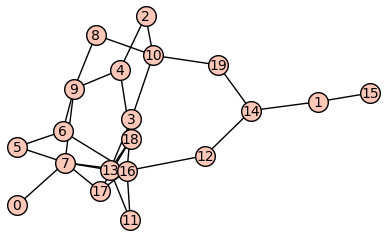
\includegraphics[width=0.5\textwidth]{Images/TreeDecomposition/bucket_elimination_graph.png}
\end{outImage}

\begin{sageCell}
    T, B = bucket_elimination(G)
\end{sageCell}
\begin{sageCell}
    T.plot()
\end{sageCell}
\begin{outImage}
   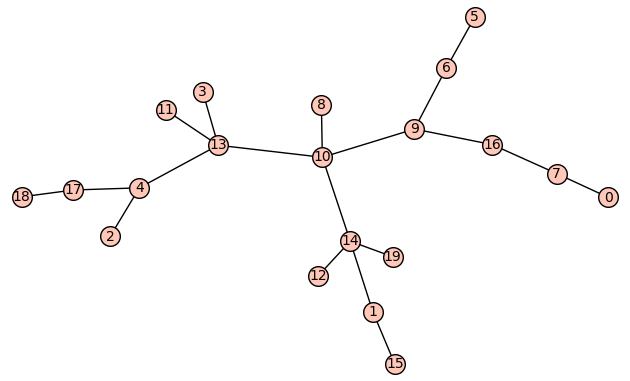
\includegraphics[width=0.5\textwidth]{Images/TreeDecomposition/bucket_elimination.png}
\end{outImage}

\begin{sageCell}
    B
\end{sageCell}
\begin{outCell}
    {7: {7},
     16: {7, 16},
     9: {7, 9, 16},
     10: {7, 9, 10, 16},
     13: {7, 9, 10, 13, 16},
     3: {3, 10, 13, 16},
     4: {4, 7, 9, 10, 13, 16},
     6: {6, 7, 9, 16},
     14: {10, 14, 16},
     17: {4, 7, 13, 16, 17},
     18: {4, 13, 17, 18},
     1: {1, 14},
     2: {2, 4, 10},
     5: {5, 6, 7},
     8: {8, 9, 10},
     11: {11, 13, 16},
     12: {12, 14, 16},
     19: {10, 14, 19},
     0: {0, 7},
     15: {1, 15}}
\end{outCell}

\begin{sageCell}
    decomposition_width(B)
\end{sageCell}
\begin{outCell}
    5
\end{outCell}
The result is 5, the size of the largest bucket $-1$

Compare to the built-in function returning tree width (should get less or equal than by \verb`decomposition_width`)
\begin{sageCell}
    T.treewidth()
\end{sageCell}
\begin{outCell}
    4
\end{outCell}


\subsection{Nice tree decomposition}

A \emph{nice tree decomposition} is a rooted binary tree decomposition with four kinds of tree vertices:
\begin{enumerate}
    \item \textbf{start}: leaves have bags of size 1,
    \item \textbf{introduce}: a vertex $v$ with one child $u$, the bag of $u$ contains one element less than the bag of $v$,
    \item \textbf{forget}:  a vertex $v$ with one child $u$, the bag of $u$ contains one element more than the bag of $v$,
    \item \textbf{join}: a vertex $v$ with two children, both have the same bag as $v$.
\end{enumerate}
Write function \verb`nice_tree_decomposition(G, T, B)` which transforms the tree decomposition $(T, B)$ of the graph $G$ into a "nice tree decomposition".

\subsubsection*{Solution and tests}


Auxiliary functions
\begin{sageCell}
    def DDFS(T, r):
    """Directs the tree T to the root r."""
    active = [r]
    prev = {}
    while len(active) > 0:
        v = active.pop()
        for w in T.neighbors(v):
            if w not in prev and w not in active and w != r:
                prev[w] = v
                active.append(w)
    DT = DiGraph()
    DT.add_edges(prev.items())
    return DT
\end{sageCell}

\begin{sageCell}
def nice_tree_decomposition(T, B):
    T = T.copy()
    B = dict((v, copy(b)) for (v, b) in B.items())
    ntd_handle_leaves(T, B)
    ntd_handle_edges(T, B)
    r = T.vertices(sort=False)[0]
    DT = DDFS(T, r)
    ntd_handle_multiple_children(DT, B)
    return DT, B

def new_vertex(G):
    """Returns integer v such that v, v + 1, v + 2, ... can be used as new vertices in G."""
    vrt = [0] + [x for x in G.vertices(sort=False) if type(x) == type(1) or type(x) == type(int(1))]
    return max(vrt) + 1

def ntd_handle_leaves(T, B):
    """
    If a leaf has a bag of size > 1, then we add a new leaf with a bag with one element less and repeat until all leaves have bags of size 1.
    """
    leaves = [x for x in T.vertices(sort=False) if T.degree(x) == 1]
    nv = new_vertex(T)

    for l in leaves:
        A = copy(B[l])
        while len(A) > 1:
            T.add_edge((l,nv))
            A.pop()
            B[nv] = copy(A)
            l = nv
            nv = nv + 1

def ntd_handle_edges(T, B):
    nv = new_vertex(T)

    for (x, y) in T.edges(labels=False, sort=False):
        Bx = copy(B[x])
        By = copy(B[y])
        Bxy = Bx & By

        if len(By) < len(Bx):
            x, y = y, x
            Bx, By = By, Bx

        T.delete_edge((x, y))

        path = [a for a in Bx if a not in Bxy]
        while path != []:
            a = path.pop()
            T.add_edge((x, nv))
            Bx.remove(a)
            B[nv] = copy(Bx)
            x = nv
            nv = nv + 1

        path = [a for a in By if a not in Bxy]
        path.pop()
        while path != []:
            a = path.pop()
            T.add_edge((x, nv))
            Bx = Bx | set([a])
            B[nv] = copy(Bx)
            x = nv
            nv = nv + 1
        T.add_edge((x, y))

def ntd_handle_multiple_children(DT, B):
    big_vertices = [x for x in DT.vertices(sort=False) if DT.in_degree(x) > 2]
    nv = new_vertex(DT)

    while big_vertices != []:
        v = big_vertices.pop()
        Nv = DT.neighbors_in(v)
        Nv.pop()
        for u in Nv:
            DT.delete_edge((u, v))
            DT.add_edge((u, nv))
        DT.add_edge((nv, v))
        B[nv] = copy(B[v])
        if len(Nv) > 2:
            big_vertices.append(nv)
        nv = nv + 1

    big_vertices = [x for x in DT.vertices(sort=False) if DT.in_degree(x) == 2]
    for v in big_vertices:
        u,w = DT.neighbors_in(v)
        if B[u] != B[v]:
            DT.delete_edge((u, v))
            DT.add_path((u, nv, v))
            B[nv] = copy(B[v])
            nv = nv + 1
        if B[w] != B[v]:
            DT.delete_edge((w, v))
            DT.add_path((w, nv, v))
            B[nv] = copy(B[v])
            nv = nv + 1
\end{sageCell}
Example
\begin{sageCell}
    NT, NB = nice_tree_decomposition(T, B)
\end{sageCell}

\begin{sageCell}
def is_nice_tree_decomposition(G, T, B):
    if not is_tree_decomposition(G, T, B):
        return False
    for v in T.vertices(sort=False):
        nin = NT.neighbors_in(v)
        if len(nin) == 0: # leaf
            if len(B[v]) != 1:
                print(f"leaf {v} has bag of size {len(B[v])}")
                return False
        elif len(nin) > 2:
            print(f"vertex {v} has 3 or more children")
        elif len(nin) == 1:
            u = nin[0]
            ints = B[v] & B[u]
            if len(B[v] - ints) > 1 or len(B[u] - ints) > 1:
                print(f"verices {v} and {u} have bags {B[v]} and {B[u]} with difference > 1")
        # len(nin) == 2
        elif B[v] != B[nin[0]] or B[v] != B[nin[1]]:
            print(f"children of {v} have different bags")
            return False
    return True
\end{sageCell}

\begin{sageCell}
    is_nice_tree_decomposition(G, NT, NB)
\end{sageCell}
\begin{outCell}
    True
\end{outCell}

